\chapter{Evaluation}

\section{400 samples, local max pooling}
T-test probability that the AoC distributions are the same: 0.009790328758564197
T-test probability that the F1 distributions are the same: 0.011943604700946929
\begin{table}[htb]
  \centering
  \begin{tabular}{lrrrr}
    \toprule
    model & \multicolumn{2}{c}{F1} & \multicolumn{2}{c}{AoC} \\
    \cmidrule(l){2-3} \cmidrule(l){4-5}
    & mean & std & mean & std \\
    \midrule
    CNN & 0.79126 & 0.01644 & 0.856768 & 0.0219711 \\
    CNN-clusters & 0.83429 & 0.02047 & 0.904359 & 0.0168642 \\
    \bottomrule
  \end{tabular}
  \caption{Performance metrics on a small dataset (200 positive
    samples)}
  \label{tbl:small}
\end{table}

\begin{figure}[htb]
  \centering
  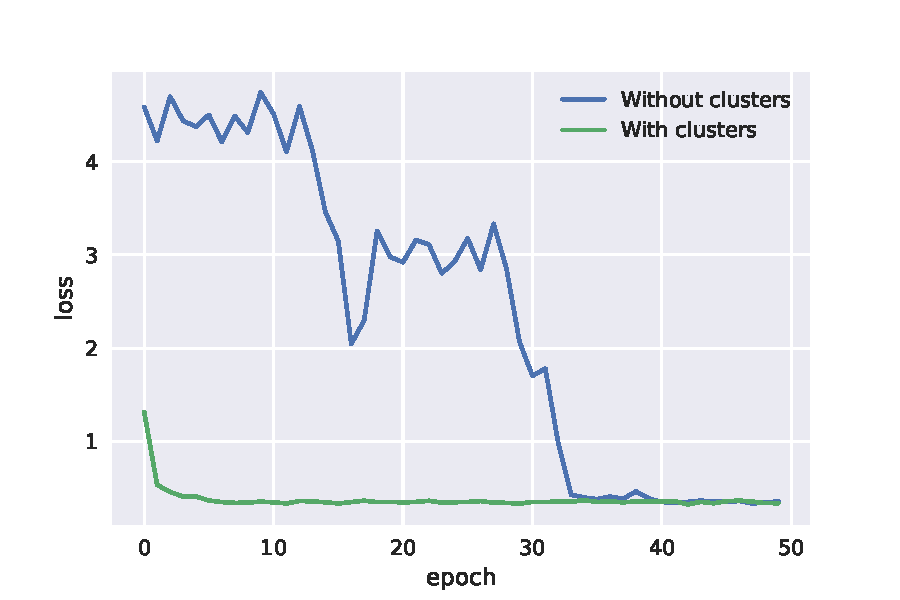
\includegraphics[width=\textwidth]{figures/results/small_5_fold_convergence.pdf}
  \caption{The convergence speed}
  \label{fig:small_convergence}
\end{figure}

\begin{figure}[htb]
  \centering
  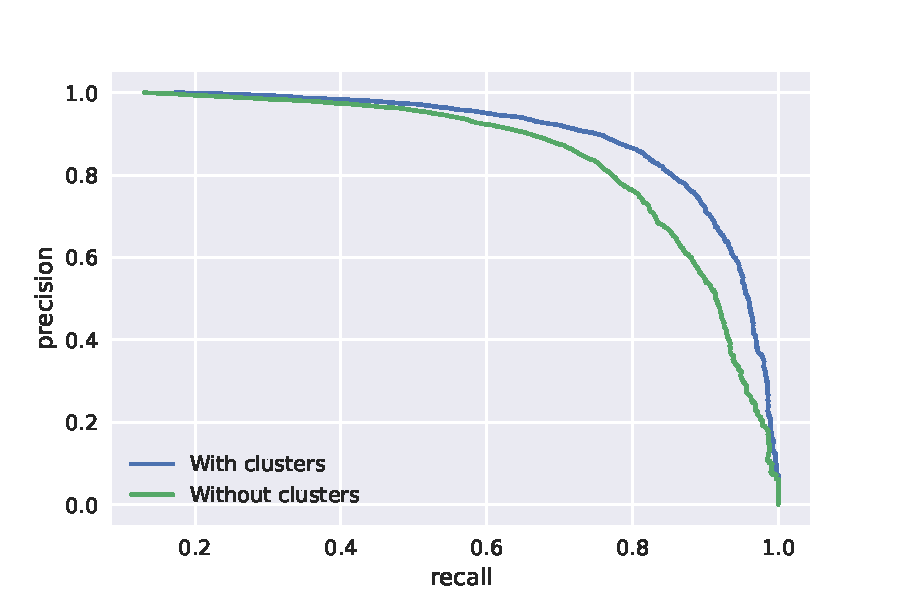
\includegraphics[width=\textwidth]{figures/results/small_5_fold_pr.pdf}
  \caption{The precision/recall curves}
  \label{fig:small_convergence}
\end{figure}

\begin{figure}[htb]
  \centering
  \begin{subfigure}[b]{0.80\textwidth} 
    \centering
    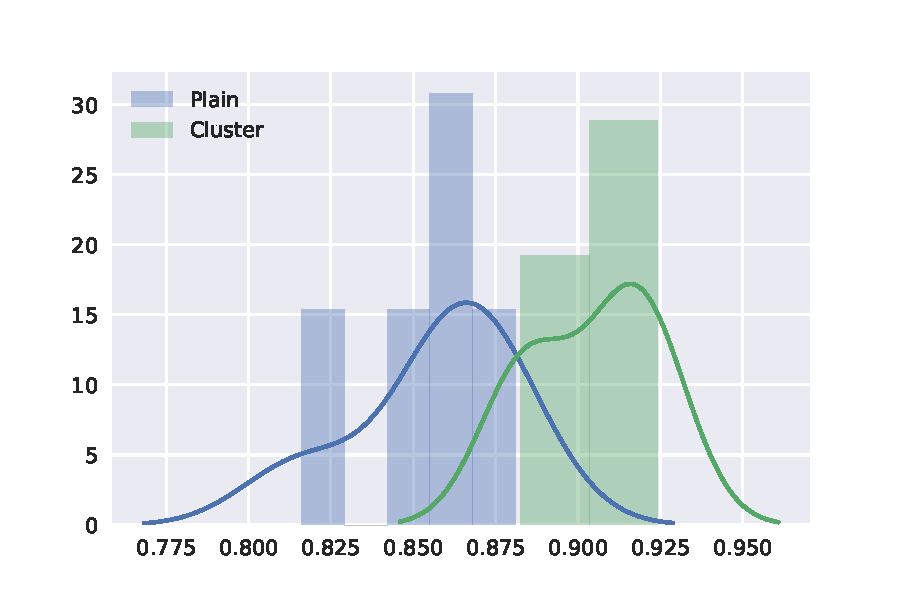
\includegraphics[width=\textwidth]{figures/results/small_5_fold_kde.pdf}
    \caption{Kernel density estimation}
  \end{subfigure}
  \vspace{0.10\textwidth}
  \begin{subfigure}[b]{0.80\textwidth}
	\centering
    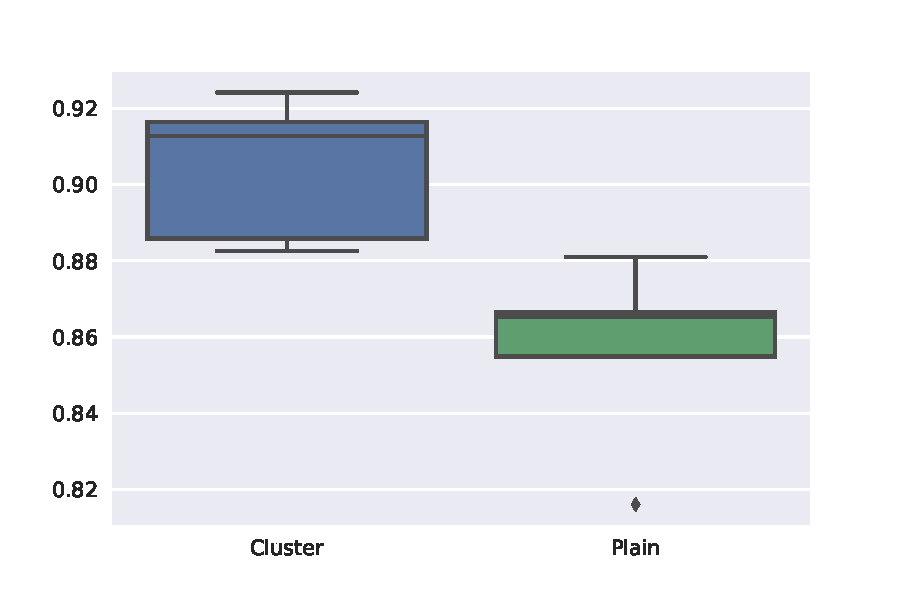
\includegraphics[width=\textwidth]{figures/results/small_5_fold_boxplot.pdf}
    \caption{Boxplot}
  \end{subfigure}
  \caption{The distribution of the cross validation results}
  \label{fig:small_dist}
\end{figure}

%%% Local Variables:
%%% mode: latex
%%% TeX-master: "report"
%%% End: